\section{Clustering}
\subsection{Unsupervised Learning}
Alles bisher war Supervised Learning. Nun ist das Thema Unsupervised Learning. Hier haben wir nur die Features (X-Werte) und uns sind die Labels (Y-Werte) unbekannt.\\
Damit können wir die Struktur der Daten lernen. Wir wollen das Pattern der Daten selbst entdecken. Die Struktur kann auch durch Noise Verborgen sein. Menschen können Struktur sehr leicht erkennen und Alogrithmen haben es schwerer. Wo uns aber Algorithmen unterstützten ist bei grossen Daten mit vielen Dimensionen. Wir können maximal 3 Dimensionen haben.
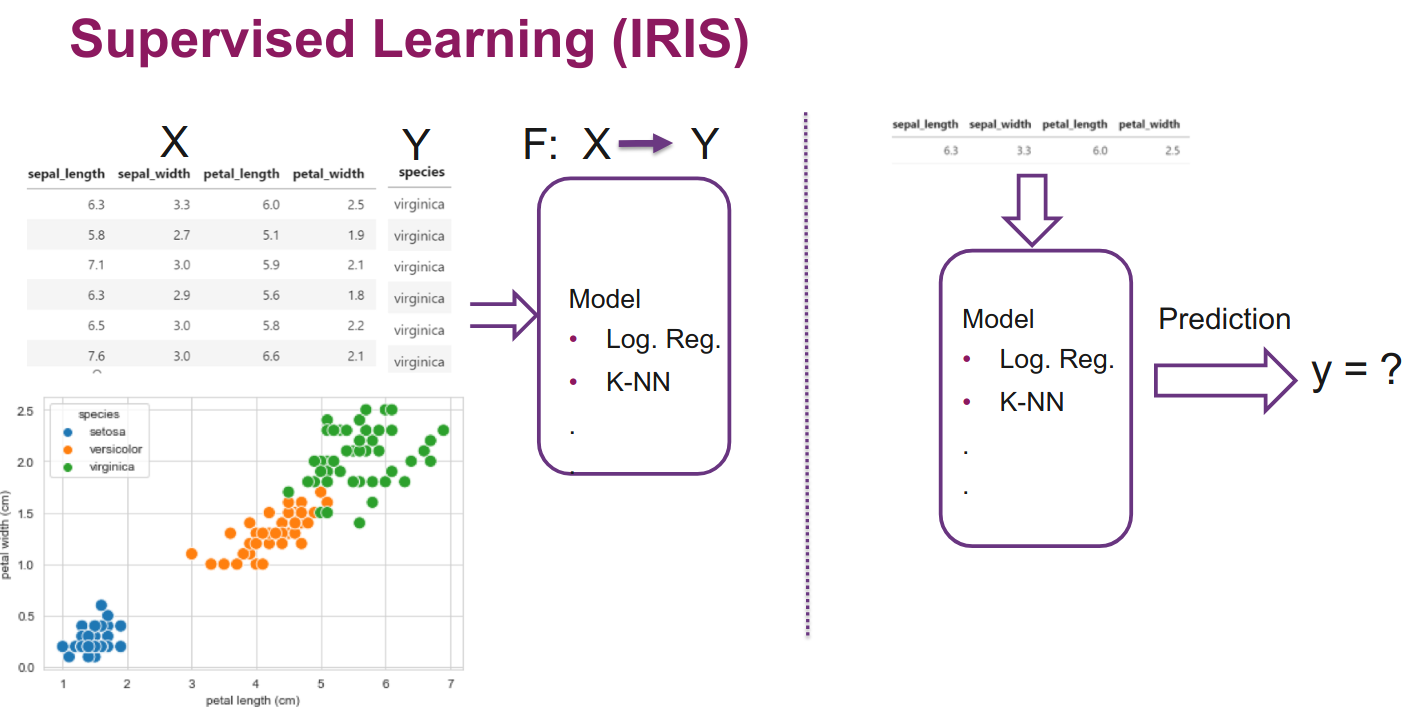
\includegraphics[width=\linewidth]{img/supervised_iris.png}
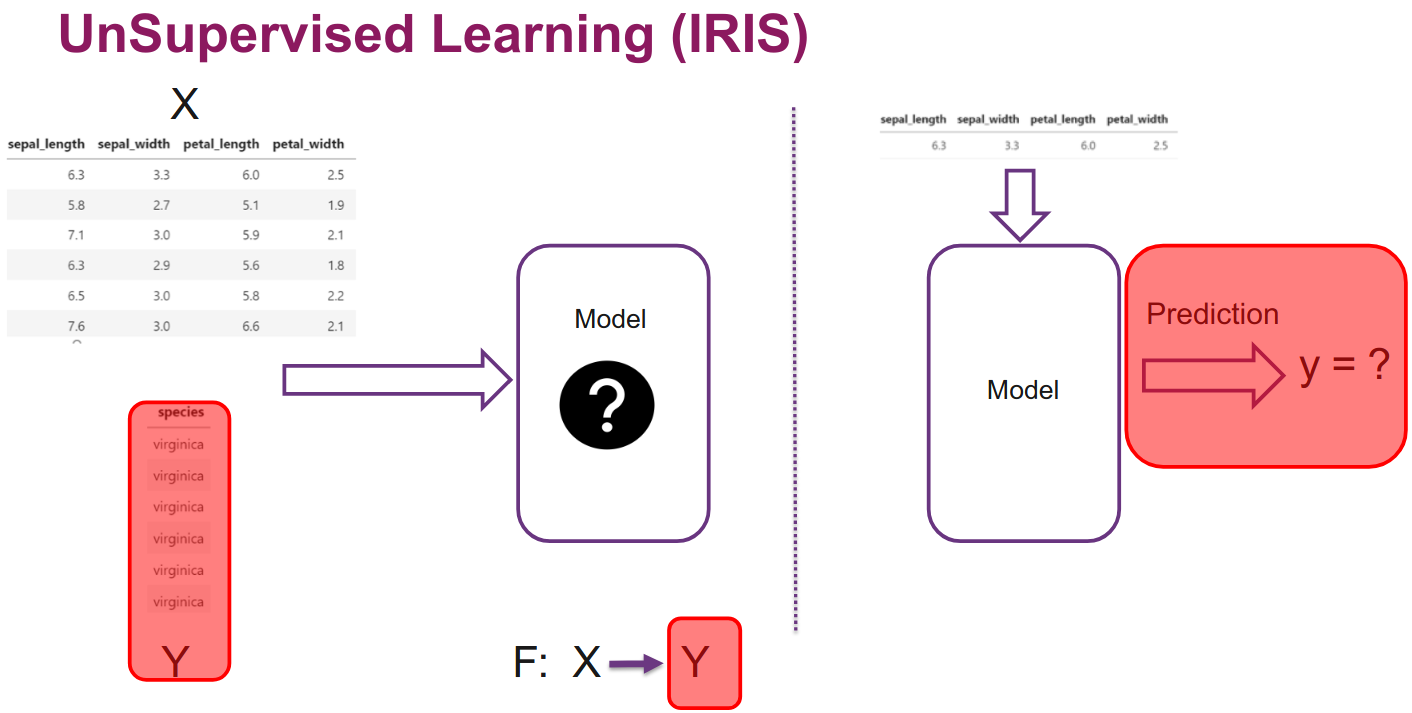
\includegraphics[width=\linewidth]{img/unsupervised_iris.png}
\subsection{Clustering (Mit KNN Klassifizierung)}
Ein Beispiel, was wir erkennen können mit unsupervised Learning sind Clusters: Datenpunkte mit ähnlichen Werten fallen in einer Gruppe zusammen.\\
\textcolor{myblue}{Beispiele:}
\begin{itemize}
\item Soziale Netzwerke analysieren
\item Astromische Daten
\item Google News (Gruppieren von News in Kategorien)
\item Market Segmentation
\end{itemize}

Wir können KNN Klassifierung zur Hilfe nehmen. Denn wir nehmen an, dass ähnliche Datenpunkte nahe zusammen sind. (Distanzmetriken: Eculidean, Manhattan)\\
\\
Group \textbf{n} data points into $k_c$ number of clusters.
\section{Naive K-means}
Ein Algorithmus um Cluster zu erkennen.
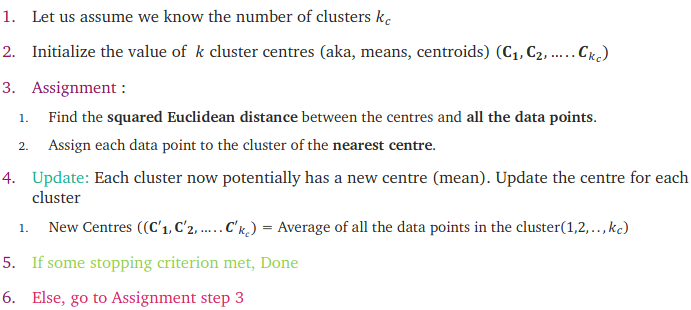
\includegraphics[width=\linewidth]{img/clustering_naive_k-means.png}
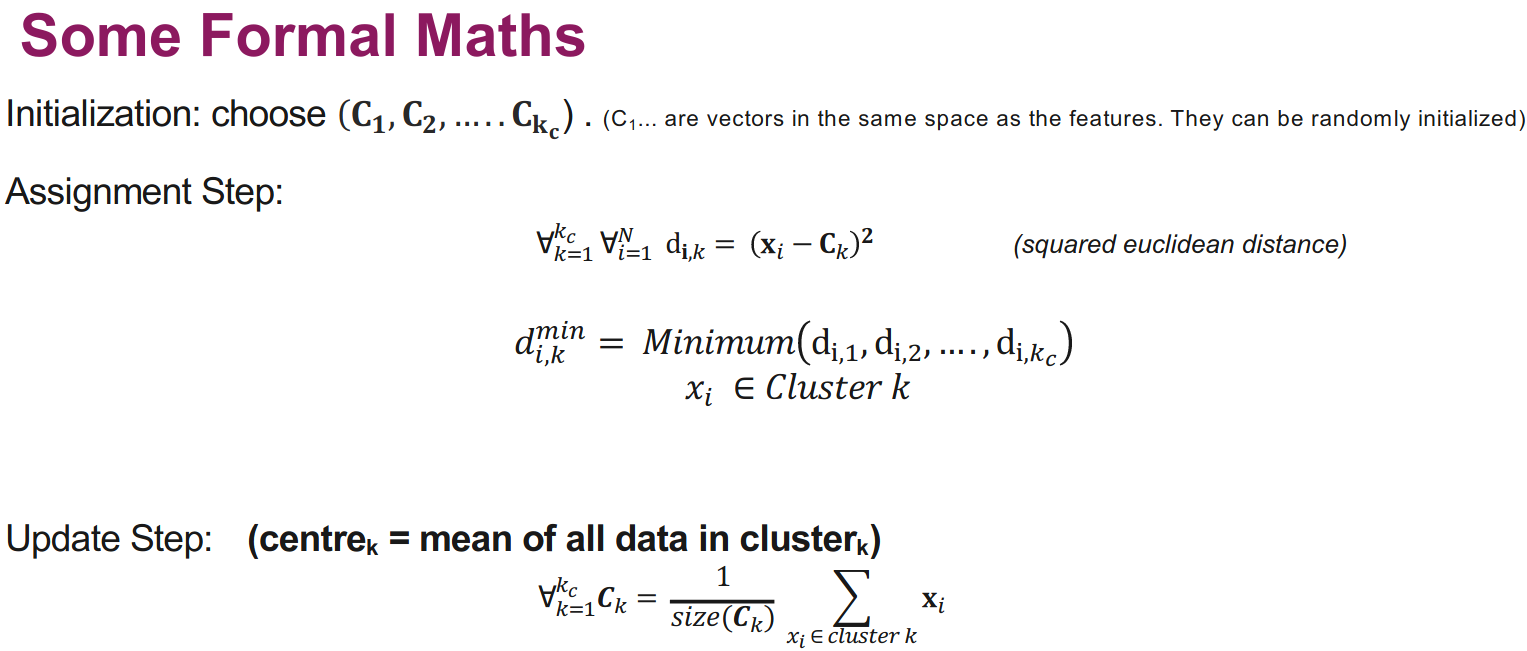
\includegraphics[width=\linewidth]{img/k-means_math.png}
\subsection{Stopping-Kriterium}
\begin{itemize}
\item Wenn «Centres» nicht mehr ändern (Zeitaufwändig)
\item Datenpunkte in einem Cluster ändern sich nicht mehr (Geht viel zu lange)
\item Distanz vom Datenpunkt zum Zentrum >= gewählten Threshold
\item Fixe Anzahl an Iterationen erreicht
\begin{itemize}
\item Zu wenig Iterationen: Schlechte Cluster -> Muss gut gewählt werden
\end{itemize}
\end{itemize}
\subsection{Intialisierung}
Die Anfangs-Zentrumswerte sind meist zufällig. Somit ist die Performance davon abhängig. Bestimmte Anfangswerte führen auch zu schlechten Convergence-Raten oder auch schlechtes Clustering. Wenn die Zentrumswerte nahe beieinander sind braucht es viel mehr Iterationen. Am besten also mehrmals ausführen und wenn Cluster stabil bleibt dann haben wir gutes Cluster.
\subsection{Standardisierung}
Die Daten müssen normalisiert werden. Ist wichtig, dass Features mit grossen Werte nicht dominieren.\\
Beispiel: Noten und Berufserfahrung. Ohne Normalisierung hat die Berufserfahrung ein Übergewicht und die Noten spielen keine Rolle.
\subsection{Qualität des Clusters: WCSS und Silhouette}
Die Nummer des Cluster ist ein Hyperparameter, der intelligent gewählt werden muss. Was man bereits im voraus sagen kann. $K_c = 1$ bringt uns nicht weiter (Alle Punkte gehören zum selben Cluster). $K_c = N$ ist viel zu gross, dann haben wir minimalen Abstand zum Zentrum, aber jeder Punkt ist ein eigenes Cluster. Bei Unsupervised Learning haben wir keine Testdaten die wir prüfen können, da wir keine Labels haben zum gegenchecken.
Somit benötigen wir andere Methoden.
\subsection{Within-Cluster Sum-of-Squares WCSS}
Distanz von den Punkten zum Zentrum muss minimalisiert werden.
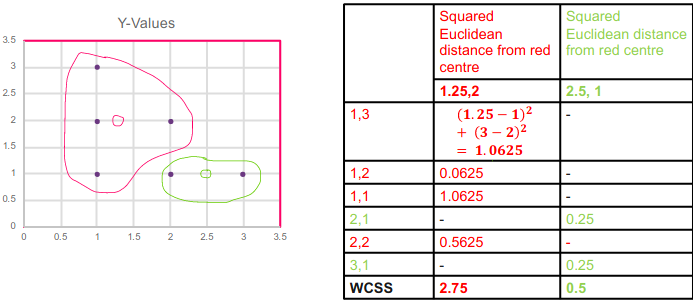
\includegraphics[width=\linewidth]{img/wcss.png}
\subsection{Silhouette Score}
Der Silhouette Score ist eine Kennzahl für die Qualität eines Clusterings. Entfernung der Punkte von einem Cluster zum anderen Cluster. Desto näher bei 1, desto besser.\\
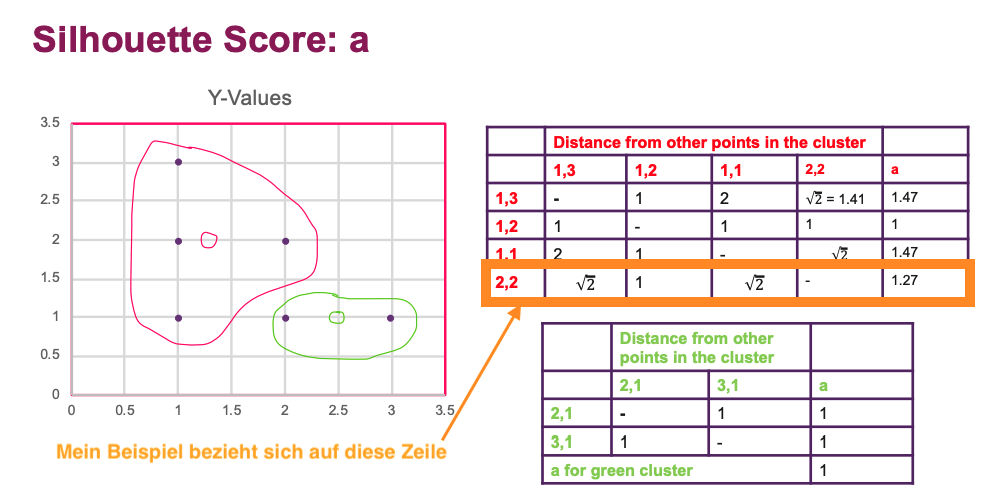
\includegraphics[width=\linewidth]{img/silhoutte_score_calculation.png}
Silhoutte Score von einem Punkt $= \frac{b-a}{max(a,b}$\\
a=Der durchschnittliche Abstand zwischen einem Punkt zu den anderen Punkten innerhalb seines eigenen Clusters.\\
b=Der Abstand zwischen einem Punkt und dem Schwerpunkt seines nächsten Nachbarclusters.\\
Für den Silhoutte Score des Clusters muss man den Durchschnitt des Scores der einzelnen Punkte im Cluster nehmen. \\
Man kann auch den Silhoutte Score des gesamten Datasets nehmen, dafür nimmt man den Durchschnitt Silhoutte Score aller Punkte. 
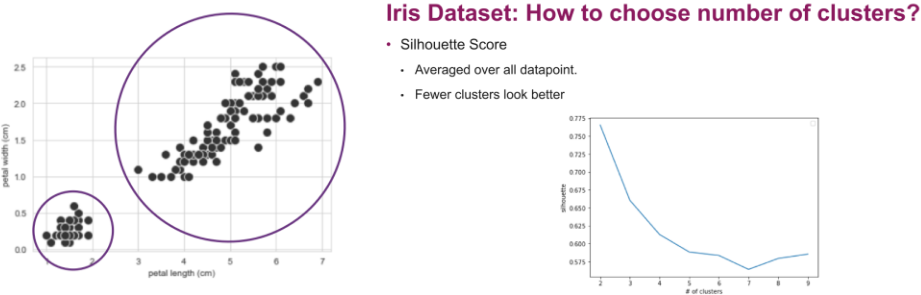
\includegraphics[width=\linewidth]{img/silhoutte_score.png}
\subsection{Bestimmung welche Clustergrösse anhand von IRIS}
In diesem Beispiel ist die optionale Clustergrösse 2-3 Cluster. Denn ab drei Cluster gibt’s beim WCSS einen Knick und es verbessert sich nicht mehr so stark. Silhouette fällt aber noch weiter.
